\documentclass[tikz,border=8pt]{standalone}
\usepackage{amsmath}
\usetikzlibrary{arrows.meta,decorations.pathreplacing}
\begin{document}
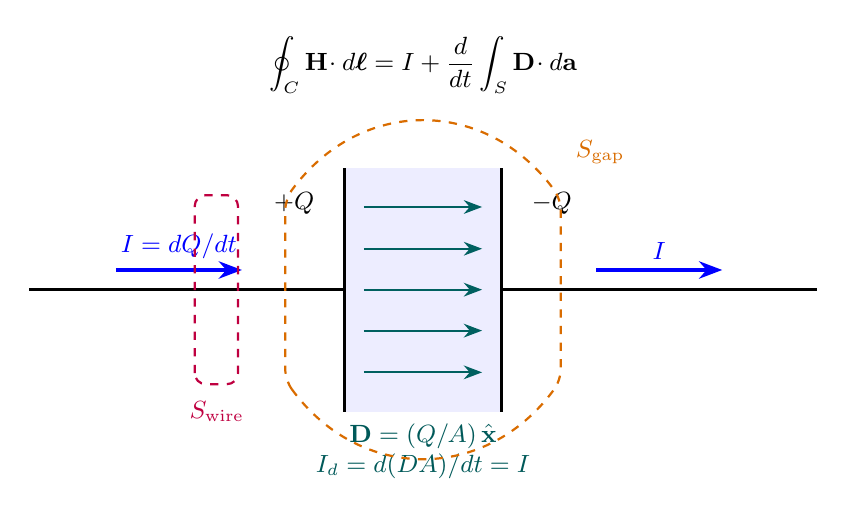
\begin{tikzpicture}[>=Stealth,font=\sffamily\small,thick]
  \fill[blue!7] (4,-1.55) rectangle (6,1.55);
  \draw[very thick] (4,-1.55)--(4,1.55) (6,-1.55)--(6,1.55);
  \draw[very thick] (0,0)--(4,0) (6,0)--(10,0);
  \foreach \y in {-1.05,-.52,0,.52,1.05}
    \draw[->,teal!75!black] (4.25,\y)--(5.75,\y);
  \draw[->,blue,very thick] (1.1,.25)--(2.7,.25)
    node[midway,above] {$I=dQ/dt$};
  \draw[->,blue,very thick] (7.2,.25)--(8.8,.25) node[midway,above] {$I$};
  \node[anchor=east] at (3.75,1.1) {$+Q$};
  \node[anchor=west] at (6.25,1.1) {$-Q$};
  \node[teal!70!black,align=center] at (5,-2.05)
    {$\mathbf D=(Q/A)\,\hat{\mathbf x}$\\$I_d=d(DA)/dt=I$};
  \draw[dashed,purple,rounded corners] (2.1,-1.2) rectangle (2.65,1.2);
  \node[purple] at (2.38,-1.55) {$S_{\rm wire}$};
  \draw[dashed,orange!85!black,rounded corners]
    (3.25,-1.15) .. controls (4.2,-2.45) and (5.8,-2.45) .. (6.75,-1.15)
    -- (6.75,1.15) .. controls (5.8,2.45) and (4.2,2.45) .. (3.25,1.15) -- cycle;
  \node[orange!85!black] at (7.25,1.75) {$S_{\rm gap}$};
  \node[align=center] at (5,2.85)
    {$\displaystyle \oint_C\mathbf H\!\cdot d\boldsymbol\ell
      =I+\frac{d}{dt}\int_S\mathbf D\!\cdot d\mathbf a$};
\end{tikzpicture}
\end{document}
